\documentclass{beamer}

\title{Load Balancing for ALICE}
\subtitle{Software for Science, CERN}

\usetheme{Berkeley}
\usecolortheme{beetle}
\begin{document}

\beamertemplatenavigationsymbolsempty
\def\logo{%
  
\includegraphics[width=2cm]{./graphics/logo.png}%
}

\setbeamertemplate{footline}{
  \begin{minipage}[t]{0.9\paperwidth}
    \hfill
    \begin{beamercolorbox}[wd=1cm, ht = 0.1cm]{page number in head/foot}
      \logo
    \end{beamercolorbox}
  \end{minipage}
}

	\frame {
		\titlepage
	}
	\frame {
		\frametitle{Index}
		\begin{itemize}
			\item Load Balancing
			\item Cluster
			\item Experiments
			\begin{itemize}
			\item Experiment 1
			\item Experiment 2
			\item Experiment 3
			\item Experiment 4
			\end{itemize}
		\end{itemize}
	}
	\frame{
		\frametitle{Load Balancing}
		\begin{columns}[T]
		\begin{column}{0.5\textwidth}
		~\\~\\~\\~\\~\\
		\begin{itemize}
			\item Setup
			\item Blacklist Algorithm
		\end{itemize}
		\end{column}
		\begin{column}{0.5\textwidth}
		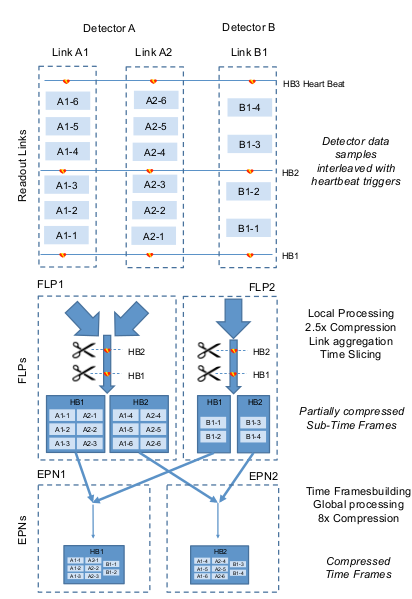
\includegraphics[scale=0.3]{./graphics/data_aggregation.png}
		\end{column}
		\end{columns}
		\footnote{Technical Design Report for the Upgrade of the Online Offline Computing System, 2015, p. 34}
	}
	\frame{
	    \frametitle{Cluster}
	    \begin{columns}[T]
	    \begin{column}{0.5\textwidth}
		~\\~\\
		\begin{itemize}
			\item Raspberry Pi
		\end{itemize}
	    \end{column}
	    \begin{column}{0.5\textwidth}
%	    \includegraphics[scale=•]{•}
	    \end{column}
	    \end{columns}
	}
	\frame{
		\frametitle{Experiments}
		\begin{itemize}
			\item Ratio
			\item Compare
			\item Expand
		\end{itemize}
	}
	\frame{
		\frametitle{Experiments}
		\framesubtitle{Experiment 1}
		\begin{columns}[T]
		
		\begin{column}{0.5\textwidth}
		~\\~\\~\\~\\~\\
		\begin{itemize}
			\item Definition
		\end{itemize}
		Ticktime influence on the Blacklist algorithm with one fail-over
		\end{column}
		
		\begin{column}{0.5\textwidth}
		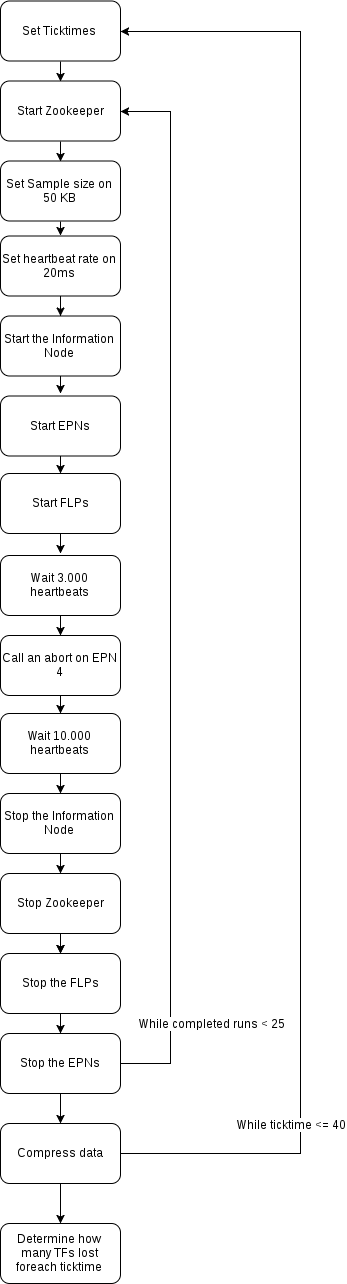
\includegraphics[scale=0.15]{./graphics/ex1.png}
		\end{column}
		
		\end{columns}
		\footnote{Effects of the EPNs and FLPs on the Information Node for ALICE, 2018, p. 19}
	}
	\frame{
		\frametitle{Experiments}
		\framesubtitle{Experiment 2}
		\begin{columns}[T]
		
		\begin{column}{0.5\textwidth}
		~\\~\\~\\~\\~\\
		\begin{itemize}
			\item Definition
		\end{itemize}
		Ticktime influence on the Blacklist algorithm with all but one fail-over
		\end{column}
		
		\begin{column}{0.5\textwidth}
		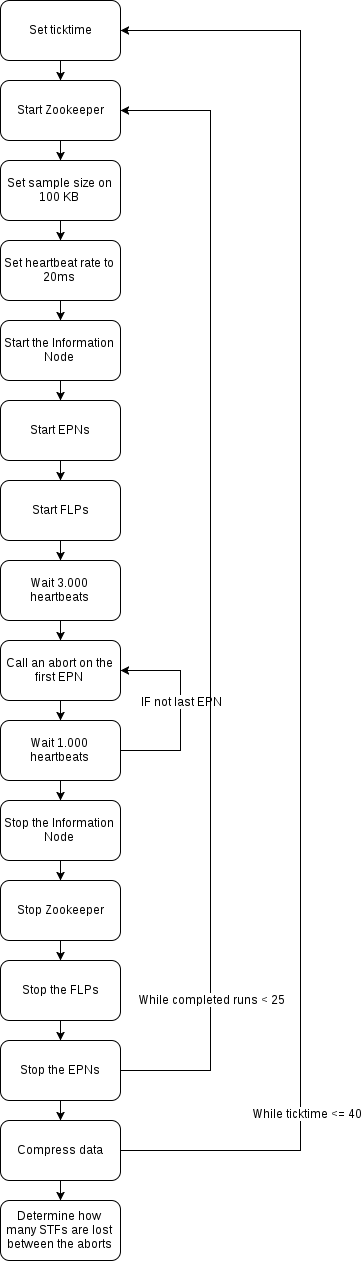
\includegraphics[scale=0.15]{./graphics/ex2.png}
		\end{column}
		
		\end{columns}
		\footnote{Effects of the EPNs and FLPs on the Information Node for ALICE, 2018, p. 20}
	}
	\frame{
		\frametitle{Experiments}
		\framesubtitle{Experiment 3}
		\begin{columns}[T]
		
		\begin{column}{0.5\textwidth}
		~\\~\\~\\~\\~\\
		\begin{itemize}
			\item Definition
		\end{itemize}
		Ticktime influence on the Blacklist algorithm with all but one fail-over using a random sample size
		\end{column}
		
		\begin{column}{0.5\textwidth}
		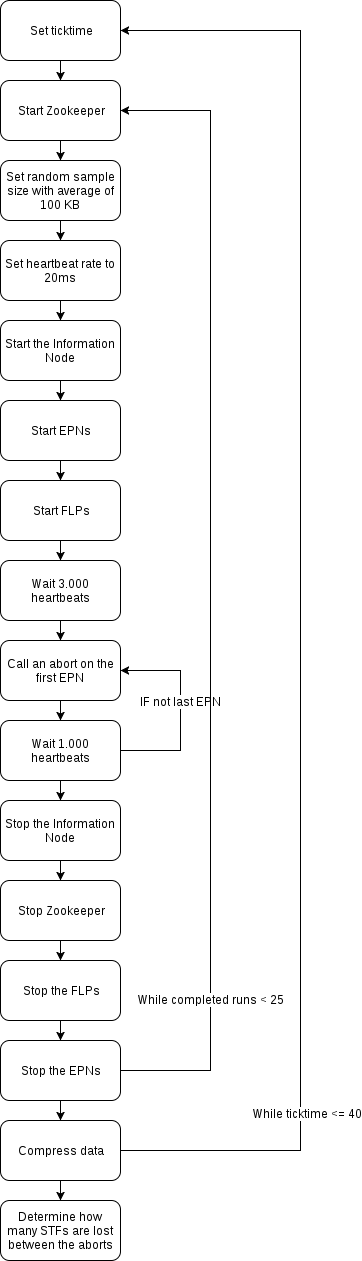
\includegraphics[scale=0.15]{./graphics/ex3.png}
		\end{column}
		
		\end{columns}		
		\footnote{Effects of the EPNs and FLPs on the Information Node for ALICE, 2018, p. 21}
	}
	\frame{
		\frametitle{Experiments}
		\framesubtitle{Experiment 4}
		\begin{columns}[T]
		
		\begin{column}{0.5\textwidth}
		~\\~\\~\\~\\~\\
		\begin{itemize}
			\item Definition
		\end{itemize}
		Ticktime influence on the Blacklist algorithm with all but one fail-over at once
		\end{column}
		
		\begin{column}{0.5\textwidth}
		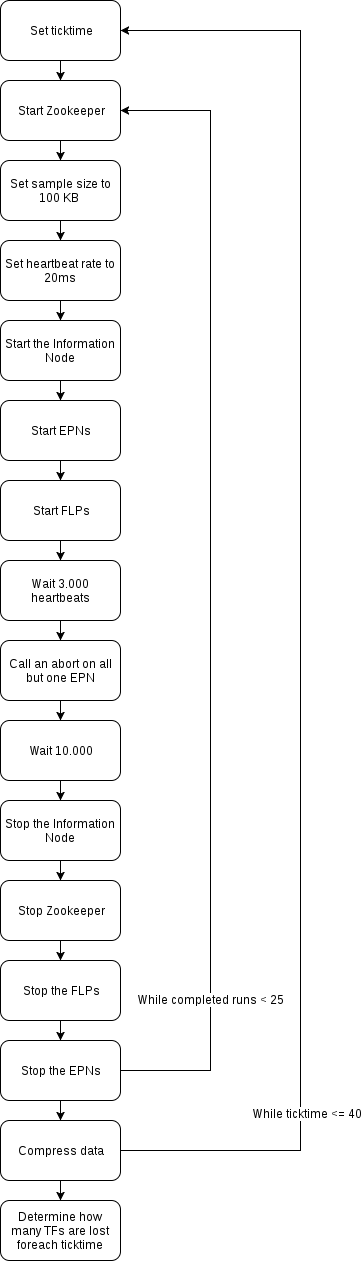
\includegraphics[scale=0.15]{./graphics/ex4.png}
		\end{column}
		
		\end{columns}
		\footnote{Effects of the EPNs and FLPs on the Information Node for ALICE, 2018, p. 22}
	}
	\frame{
		\frametitle{The end}
		Any questions perhaps?
	}
\end{document}